\chapter{Méthodes Quasi-Newton}
\label{chap:quasi-newton}

\section{Introduction}

\paragraph{Principe.}
L'objectif est d'éviter le calcul de la Hessienne en utilisant à la place une matrice symétrique définie positive.

\paragraph{Domaine d'application.}
Dans ce chapitre, nous nous concentrons sur des problèmes de taille petite à moyenne. En effet, ces méthodes nécessitent des résolutions de systèmes linéaires ; la question des grands problèmes est reportée au chapitre suivant, où on évitera de telles résolutions.

\section{La méthode BFGS}
\label{sec:bfgs}

La méthode de \textbf{Broyden, Fletcher, Goldfarb, Shanno} (BFGS) est la plus populaire des méthodes Quasi-Newton.

Considérons le modèle quadratique suivant de la fonction objectif $f$ à l'itération $k$ :
\begin{equation}
    m_k(p) = f_k + \nabla f_k^\top p + \frac{1}{2} p^\top B_k p,
\end{equation}
où $B_k$ est une matrice symétrique définie positive qui est mise à jour à chaque itération.

Notons que le modèle vérifie les propriétés de consistance suivantes en $p=0$ :
\begin{itemize}
    \item $m_k(0) = f_k = f(x_k)$
    \item $\nabla m_k(0) = \nabla f_k = \nabla f(x_k)$
\end{itemize}

Le minimiseur $p_k$ du modèle quadratique $m_k$ est obtenu en annulant son gradient :
\begin{equation}
    \nabla m_k(p_k) = \nabla f_k + B_k p_k = 0.
\end{equation}
Ceci implique que la direction de recherche est donnée par :
\begin{equation}
    p_k = -B_k^{-1} \nabla f_k.
\end{equation}

Une fois la direction $p_k$ obtenue, nous effectuons une recherche linéaire (line search) pour déterminer le pas $\alpha_k$.

\section{La formule de mise à jour de Davidon, Fletcher, Powell (DFP)}
\label{sec:dfp}

Davidon (1959) a proposé de mettre à jour $B_k$ pour prendre en compte le changement de courbure survenu depuis la dernière itération.

Considérons le nouveau modèle affiné en $x_{k+1}$ :
\begin{equation}
    m_{k+1}(p) = f_{k+1} + \nabla f_{k+1}^\top p + \frac{1}{2} p^\top B_{k+1} p.
\end{equation}

Quelles sont les exigences raisonnables pour mettre à jour $B_k$ ?

\subsection{L'équation sécante}

Par exemple, le gradient de $m_{k+1}$ doit coïncider avec le vrai gradient de $f$ aux points $x_{k+1}$ et $x_k$.

\begin{enumerate}
    \item En $x_{k+1}$ (c'est-à-dire pour $p=0$) :
    \[ \nabla m_{k+1}(0) = \nabla f_{k+1}. \]
    Cette condition est vérifiée par définition.

    \item En $x_k$ (c'est-à-dire pour le déplacement inverse $p = -\alpha_k p_k$) :
    Nous voulons que :
    \begin{equation}
        \nabla m_{k+1}(-\alpha_k p_k) = \nabla f_{k+1} + B_{k+1}(-\alpha_k p_k) = \nabla f_k.
    \end{equation}
\end{enumerate}

Réarrangeons cette dernière équation :
\[
    B_{k+1} (\alpha_k p_k) = \nabla f_{k+1} - \nabla f_k.
\]

Introduisons les vecteurs $s_k$ (déplacement) et $y_k$ (changement de gradient) :
\begin{align}
    s_k &= x_{k+1} - x_k = \alpha_k p_k, \\
    y_k &= \nabla f_{k+1} - \nabla f_k.
\end{align}

On obtient alors l'\textbf{équation sécante} :
\begin{equation}
    \label{eq:secant}
    B_{k+1} s_k = y_k.
\end{equation}
La matrice $B_{k+1}$ doit transformer $s_k$ en $y_k$.

\begin{figure}[H]
\centering
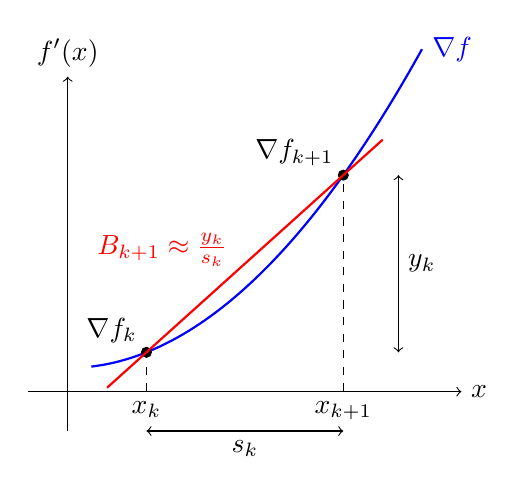
\begin{tikzpicture}[scale=1.0]
    % Axes
    \draw[->] (-0.5,0) -- (5,0) node[right] {$x$};
    \draw[->] (0,-0.5) -- (0,4) node[above] {$f'(x)$};
    
    % Derivative curve f'(x) - convex increasing: f'(x) = 0.2*x^2 + 0.3
    % At x=1: f'(1) = 0.2*1 + 0.3 = 0.5
    % At x=3.5: f'(3.5) = 0.2*12.25 + 0.3 = 2.45 + 0.3 = 2.75
    \draw[domain=0.3:4.5, smooth, variable=\x, blue, thick] 
        plot ({\x}, {0.2*\x*\x + 0.3}) node[right] {$\nabla f$};
    
    % Points x_k and x_{k+1}
    \coordinate (xk) at (1, 0);
    \coordinate (xk1) at (3.5, 0);
    \coordinate (fk) at (1, 0.5);
    \coordinate (fk1) at (3.5, 2.75);
    
    % Vertical lines to curve
    \draw[dashed] (1, 0) -- (fk);
    \draw[dashed] (3.5, 0) -- (fk1);
    
    % Points on curve
    \fill (fk) circle (2pt);
    \fill (fk1) circle (2pt);
    
    % Secant line - must pass through (1, 0.5) and (3.5, 2.75)
    % Slope = (2.75 - 0.5) / (3.5 - 1) = 2.25 / 2.5 = 0.9
    % At x=0.5: y = 0.5 + 0.9*(0.5 - 1) = 0.5 - 0.45 = 0.05
    % At x=4: y = 0.5 + 0.9*(4 - 1) = 0.5 + 2.7 = 3.2
    \draw[red, thick] (0.5, 0.05) -- (4, 3.2);
    
    % Labels
    \node[below] at (1, 0) {$x_k$};
    \node[below] at (3.5, 0) {$x_{k+1}$};
    \node[above left] at (fk) {$\nabla f_k$};
    \node[above left] at (fk1) {$\nabla f_{k+1}$};
    
    % Brace for s_k - lowered
    \draw[<->] (1, -0.5) -- (3.5, -0.5) node[midway, below] {$s_k$};
    
    % Brace for y_k
    \draw[<->] (4.2, 0.5) -- (4.2, 2.75) node[midway, right] {$y_k$};
    
    % Secant slope annotation - positioned upper left of red line
    \node[red] at (1.2, 1.8) {$B_{k+1} \approx \frac{y_k}{s_k}$};
\end{tikzpicture}
\caption{Interprétation géométrique de l'équation sécante (cas 1D) : $B_{k+1}$ est la pente de la sécante de la courbe $\nabla f$.}
\label{fig:secant-geometry}
\end{figure}

\begin{figureexplanation}
La figure~\ref{fig:secant-geometry} illustre le principe de l'équation sécante en dimension 1. La matrice (ici un scalaire) $B_{k+1}$ correspond à la pente de la droite sécante (en rouge) reliant les points $(\nabla f_k, x_k)$ et $(\nabla f_{k+1}, x_{k+1})$ sur la courbe du gradient (en bleu). Cette pente approxime la courbure moyenne de la fonction entre ces deux points.
\end{figureexplanation}

\subsection{Condition de courbure}

Une condition nécessaire pour que $B_{k+1}$ soit définie positive (comme nous le souhaitons pour avoir une direction de descente) est obtenue en multipliant l'équation sécante par $s_k^\top$ à gauche :
\[
    s_k^\top B_{k+1} s_k = s_k^\top y_k.
\]
Si $B_{k+1} \succ 0$, alors on doit avoir :
\begin{equation}
    s_k^\top y_k > 0.
\end{equation}
C'est ce qu'on appelle la \textbf{condition de courbure}.

\begin{itemize}
    \item Cette condition est toujours satisfaite si $f$ est fortement convexe.
    \item Sinon, nous devons l'imposer en appliquant les \textbf{conditions de Wolfe} lors de la recherche linéaire (line search).
\end{itemize}

\subsubsection{Preuve avec les conditions de Wolfe}

La seconde condition de Wolfe est :
\begin{equation}
    \nabla f_{k+1}^\top p_k \ge c_2 \nabla f_k^\top p_k.
\end{equation}
Comme $s_k = \alpha_k p_k$ avec $\alpha_k > 0$, cela équivaut à :
\[
    \nabla f_{k+1}^\top s_k \ge c_2 \nabla f_k^\top s_k.
\]
Ainsi :
\begin{align*}
    y_k^\top s_k
    &= (\nabla f_{k+1} - \nabla f_k)^\top s_k \\
    &\ge c_2 \nabla f_k^\top s_k - \nabla f_k^\top s_k \\
    &= (c_2 - 1) \nabla f_k^\top s_k \\
    &= (c_2 - 1) \alpha_k \nabla f_k^\top p_k.
\end{align*}
Comme $c_2 < 1$ (donc $c_2 - 1 < 0$) et que $p_k$ est une direction de descente ($\nabla f_k^\top p_k < 0$), le produit est strictement positif :
\[
    y_k^\top s_k > 0.
\]

\subsection{Construction de la mise à jour DFP}

L'équation sécante $B_{k+1} s_k = y_k$ admet une infinité de solutions (car $B_{k+1}$ a $n(n+1)/2$ degrés de liberté pour seulement $n$ contraintes).

Nous avons besoin d'un autre critère : choisir $B_{k+1}$ le plus « proche » possible de $B_k$.
On résout :
\begin{equation}
    B_{k+1} = \arg\min_B \|B - B_k\| \quad \text{t.q. } B=B^\top \text{ et } B s_k = y_k.
\end{equation}

DFP a choisi la norme de Frobenius pondérée :
\[
    \|A\|_W = \|W^{1/2} A W^{1/2}\|_F, \quad \text{où } \|C\|_F^2 = \sum_{i,j} C_{ij}^2.
\]
La matrice de pondération $W$ est choisie telle que $W y_k = s_k$.

Par exemple, on peut choisir $W = (\bar{G}_k)^{-1}$, où $\bar{G}_k$ est la Hessienne moyenne :
\[
    \bar{G}_k = \int_0^1 \nabla^2 f(x_k + \tau \alpha_k p_k) d\tau.
\]
D'après le théorème de Taylor :
\[
    \nabla f(x_{k+1}) = \nabla f(x_k) + \bar{G}_k (x_{k+1} - x_k),
\]
c'est-à-dire $y_k = \bar{G}_k s_k$, ce qui correspond bien au choix de $W$.

Avec ce choix de $W$, la solution est donnée par la formule de mise à jour DFP :
\begin{equation}
    \label{eq:dfp-formula}
    B_{k+1} = (I - \rho_k y_k s_k^\top) B_k (I - \rho_k s_k y_k^\top) + \rho_k y_k y_k^\top,
\end{equation}
où
\begin{equation}
    \rho_k = \frac{1}{y_k^\top s_k}.
\end{equation}

\subsection{Expression de l'inverse (Formule de Sherman-Morrison-Woodbury)}

Si on exprime la mise à jour en termes de l'inverse de la Hessienne $H_k = B_k^{-1}$, comme dans la méthode de Newton où $p_k = -H_k \nabla f_k$, on peut utiliser la formule de Sherman-Morrison-Woodbury.

La formule de mise à jour DFP pour l'inverse est donnée par :
\begin{equation}
    H_{k+1}^{DFP} = H_k - \frac{H_k y_k y_k^\top H_k}{y_k^\top H_k y_k} + \frac{s_k s_k^\top}{y_k^\top s_k}.
\end{equation}
On remarque que cette mise à jour correspond à l'ajout de deux matrices de rang 1 (mise à jour de rang 2).
De plus, $\text{rang}(H_{k+1} - H_k) \le 2$.

\section{L'approche BFGS}
\label{sec:bfgs_approach}

La méthode BFGS (Broyden-Fletcher-Goldfarb-Shanno) utilise le même raisonnement que DFP, mais en travaillant directement sur l'inverse de la Hessienne $H_k$ au lieu de $B_k$.

L'équation sécante pour l'inverse devient :
\begin{equation}
    H_{k+1} y_k = s_k.
\end{equation}
On cherche alors $H_{k+1}$ solution de :
\begin{equation}
    H_{k+1} = \arg\min_H \|H - H_k\|_W \quad \text{t.q. } H=H^\top \text{ et } H y_k = s_k.
\end{equation}
La solution donne la \textbf{formule de mise à jour BFGS} pour l'inverse :
\begin{equation}
    H_{k+1}^{BFGS} = (I - \rho_k s_k y_k^\top) H_k (I - \rho_k y_k s_k^\top) + \rho_k s_k s_k^\top,
\end{equation}
avec $\rho_k = \frac{1}{y_k^\top s_k}$.

\begin{algorithm}[H]
\caption{Méthode BFGS}
\label{alg:bfgs}
Given starting point $x_0$, convergence tolerance $\varepsilon > 0$, inverse Hessian approximation $H_0$\;
$k \leftarrow 0$\;
\While{$\|\nabla f_k\| > \varepsilon$}{
    Compute search direction $p_k = -H_k \nabla f_k$\;
    Set $x_{k+1} = x_k + \alpha_k p_k$, where $\alpha_k$ is computed from a line search procedure to satisfy the Wolfe conditions\;
    $s_k \leftarrow x_{k+1} - x_k$\;
    $y_k \leftarrow \nabla f_{k+1} - \nabla f_k$\;
    Compute $H_{k+1} = (I - \rho_k s_k y_k')H_k(I - \rho_k y_k s_k') + \rho_k s_k s_k'$\;
    $k \leftarrow k + 1$\;
}
\end{algorithm}

\begin{figure}[H]
\centering

\includegraphics[width=0.7\textwidth]{4.png}
\caption{Itérations de la méthode BFGS sur les courbes de niveau de la fonction de Rosenbrock.}
\label{fig:bfgs-rosenbrock}
\end{figure}

\begin{figureexplanation}
\textbf{Points clés à observer :}
\begin{itemize}
    \item \textbf{Trajectoire directe :} Contrairement à la descente de gradient qui zigzague, BFGS converge rapidement vers le minimum $(1,1)$ en utilisant l'approximation de la courbure.
    \item \textbf{Adaptation locale :} La méthode apprend progressivement la forme de la Hessienne au fur et à mesure des itérations, ce qui lui permet de « redresser » ses directions de recherche.
    \item \textbf{Comparaison :} Le nombre d'itérations est bien inférieur à celui de la descente de gradient (Figure correspondante dans le chapitre 2), mais légèrement supérieur à Newton (qui utilise la vraie Hessienne).
\end{itemize}
\end{figureexplanation}

\section{Méthodes Quasi-Newton à mémoire limitée (L-BFGS)}
\label{sec:lbfgs}

Pour des problèmes de grande dimension, stocker la matrice $H_k$ (de taille $n \times n$) devient prohibitif.
La méthode L-BFGS (Limited-memory BFGS) résout ce problème en stockant uniquement les $m$ dernières paires $(s_k, y_k)$.

\begin{algorithm}[H]
\caption{L-BFGS récursion à deux boucles}
\label{alg:lbfgs-twoloop}
$q \leftarrow \nabla f_k$\;
\For{$i = k-1, k-2, \ldots, k-m$}{
    $\alpha_i \leftarrow \rho_i s_i' q$\;
    $q \leftarrow q - \alpha_i y_i$\;
}
$r \leftarrow H_k^0 q$\;
\For{$i = k-m, k-m+1, \ldots, k-1$}{
    $\beta \leftarrow \rho_i y_i' r$\;
    $r \leftarrow r + s_i(\alpha_i - \beta)$\;
}
\Stop with result $H_k \nabla f_k = r$.
\end{algorithm}

\begin{algorithm}[H]
\caption{L-BFGS}
\label{alg:lbfgs}
Choose starting point $x_0$, integer $m > 0$\;
$k \leftarrow 0$\;
\Repeat{convergence}{
    Choose $H_k^0$, for instance $H_k^0 = \dfrac{s_{k-1}'y_{k-1}}{y_{k-1}'y_{k-1}} I$\;
    Compute $p_k \leftarrow -H_k \nabla f_k$ from Algorithm~\ref{alg:lbfgs-twoloop}\;
    Compute $x_{k+1} \leftarrow x_k + \alpha_k p_k$, where $\alpha_k$ is chosen to satisfy the Wolfe conditions\;
    \If{$k > m$}{
        Discard the vector pair $\{s_{k-m}, y_{k-m}\}$ from storage\;
    }
    Compute and save $s_k \leftarrow x_{k+1} - x_k$, $y_k = \nabla f_{k+1} - \nabla f_k$\;
    $k \leftarrow k + 1$\;
}
\end{algorithm}

\section{Remarques et Propriétés}

\paragraph{Initialisation.} Il n'y a pas d'initialisation optimale universelle pour $H_0$.
Les possibilités sont :
\begin{itemize}
    \item Approximer la Hessienne inverse initiale.
    \item Prendre un multiple de l'identité $H_0 = \gamma I$.
\end{itemize}

\paragraph{Coût.} Le coût de calcul de chaque itération est en $O(n^2)$ (multiplications matrice-vecteur et mises à jour de rang 1/2), contrairement à $O(n^3)$ pour Newton (qui nécessite une inversion de système).

\paragraph{Définie positivité.}
Si $H_k$ est définie positive, alors $H_{k+1}$ l'est aussi, pourvu que $y_k^\top s_k > 0$.
En effet, pour tout $z \neq 0$ :
\[
    z^\top H_{k+1} z = z^\top (I - \rho s y^\top) H (I - \rho y s^\top) z + \rho (z^\top s)^2 \geq 0.
\]
En toute rigueur, à ce stade on a seulement $\geq 0$ car $(I - \rho y s^\top) z$ et $z^\top s$ pourraient être nuls. Cependant, si $z^\top s = 0$, alors il ne reste que le terme $z^\top (I - \rho s y^\top) H (I - \rho y s^\top) z$, qui est $> 0$ car $H$ est définie positive et $(I - \rho y s^\top) z \neq 0$ (sinon $z = \rho (y^\top z) s$, ce qui impliquerait $z^\top s = \rho (y^\top z) s^\top s \neq 0$, contradiction). Donc $z^\top H_{k+1} z > 0$.

\section{La classe de Broyden}

Il existe une famille de mises à jour, appelée classe de Broyden, définie par :
\begin{equation}
    B_{k+1} = (1-\phi_k) B_{k+1}^{BFGS} + \phi_k B_{k+1}^{DFP}.
\end{equation}
Ou sous une forme explicite :
\begin{equation}
    B_{k+1} = B_k - \frac{B_k s_k s_k^\top B_k}{s_k^\top B_k s_k} + \frac{y_k y_k^\top}{y_k^\top s_k} + \phi_k (s_k^\top B_k s_k) v_k v_k^\top,
\end{equation}
où $\phi_k$ est un paramètre scalaire et
\[
    v_k = \frac{y_k}{y_k^\top s_k} - \frac{B_k s_k}{s_k^\top B_k s_k}.
\]

Cas particuliers :
\begin{itemize}
    \item Si $\phi_k = 0$, on retrouve \textbf{BFGS}.
    \item Si $\phi_k = 1$, on retrouve \textbf{DFP}.
\end{itemize}

\paragraph{Classe de Broyden restreinte.}
La classe de Broyden restreinte correspond au choix $\phi_k \in [0, 1)$.
Les méthodes de cette classe sont des combinaisons convexes de BFGS et DFP.

\section{Propriétés sur les fonctions quadratiques}

Considérons une fonction fortement quadratique $f(x) = \frac{1}{2} x^\top Q x - b^\top x$.
Supposons que $B_0$ est symétrique définie positive et que $\alpha_k$ est le pas exact (exact line search).

On a alors les propriétés suivantes (Théorème admis) :
\begin{enumerate}
    \item Les itérés $x_k$ générés sont indépendants du choix de $\phi_k$ dans la classe de Broyden.
    \item L'équation sécante est satisfaite pour toutes les directions de recherche précédentes :
    \begin{equation}
        B_k s_j = y_j, \quad \forall j = 0, \dots, k-1.
    \end{equation}
    \item Si on choisit $B_0 = I$, alors les itérés sont identiques à ceux de la méthode du gradient conjugué, et les directions de recherche sont conjuguées :
    \begin{equation}
        s_j^\top Q s_k = 0, \quad \forall j \neq k.
    \end{equation}
    \item Si on effectue $n$ itérations, alors la matrice Hessienne est identifiée exactement :
    \begin{equation}
        B_n = Q.
    \end{equation}
\end{enumerate}

\section{Analyse de convergence}

\subsection{Convergence globale}

\paragraph{Remarque.}
BFGS et les méthodes de la classe de Broyden restreinte ($\phi_k \in [0, 1)$) sont très robustes en pratique.
Cependant, il n'existe pas de résultat de convergence globale pour des fonctions non-linéaires générales (non convexes).

Nous allons énoncer un résultat pour les fonctions convexes.

\paragraph{Hypothèses B.}
\begin{itemize}
    \item La fonction objective $f$ est deux fois continûment différentiable ($C^2$).
    \item L'ensemble de niveau $\mathcal{L} = \{ x \in \mathbb{R}^n \mid f(x) \le f(x_0) \}$ est convexe.
    \item Il existe des constantes $0 < m \le M$ telles que pour tout $z \in \mathbb{R}^n$ et pour tout $x \in \mathcal{L}$ :
    \begin{equation}
        m \|z\|^2 \le z^\top \nabla^2 f(x) z \le M \|z\|^2.
    \end{equation}
\end{itemize}
Cela implique que $f$ est fortement convexe sur $\mathcal{L}$.

\begin{theoreme}[Convergence globale de BFGS]
    Soit $B_0$ une matrice symétrique définie positive quelconque.
    Soit $x_0$ un point tel que les Hypothèses B sont vérifiées.
    Alors la suite des itérés $(x_k)$ générée par l'algorithme BFGS (avec $\epsilon = 0$) converge vers le minimiseur $x^\star$ de $f$ (qui est unique d'après les Hypothèses B).
\end{theoreme}

\paragraph{Preuve.} Voir \textit{\cite{nocedal2006numerical}}.

\paragraph{Remarque.}
Ce théorème peut être généralisé à toute la classe de Broyden restreinte.

\subsection{Convergence super-linéaire de BFGS}

Il est également possible de prouver que la convergence est suffisamment rapide pour que :
\[
    \sum_{k=0}^\infty \|x_k - x^\star\| < \infty.
\]

\paragraph{Hypothèse C.}
La matrice Hessienne $G = \nabla^2 f$ est Lipschitz continue en $x^\star$ : il existe $L > 0$ tel que pour $x$ suffisamment proche de $x^\star$ :
\[
    \| \nabla^2 f(x) - \nabla^2 f(x^\star) \| \le L \| x - x^\star \|.
\]

\begin{theoreme}[Admis]
    Supposons que $f$ est deux fois continûment différentiable ($C^2$).
    Considérons les itérés $x_{k+1} = x_k + \alpha_k p_k$ où $\alpha_k$ satisfait les conditions de Wolfe avec $c_1 \le \frac{1}{2}$.
    Si la suite $(x_k)$ converge vers un point $x^\star$ où $\nabla f(x^\star) = 0$ et $\nabla^2 f(x^\star)$ est définie positive.
    Et si les directions de recherche satisfont (Condition de Dennis-Moré) :
    \begin{equation}
        \lim_{k \to \infty} \frac{\| \nabla f_k + \nabla^2 f_k p_k \|}{\| p_k \|} = 0,
    \end{equation}
    alors la valeur $\alpha_k = 1$ est admissible pour tout $k \ge k_0$ (où $k_0$ est un certain entier),
    et si on choisit $\alpha_k = 1$ pour $k \ge k_0$, la convergence de $(x_k)$ vers $x^\star$ est \textbf{super-linéaire}.
\end{theoreme}

\paragraph{Remarque.}
Si $p_k = -B_k^{-1} \nabla f_k$ est une direction quasi-Newton, alors la condition ci-dessus se réécrit :
\[
    \lim_{k \to \infty} \frac{\| (B_k - \nabla^2 f(x_k)) p_k \|}{\| p_k \|} = 0.
\]
\bigskip
\begin{checkpoint}
\begin{itemize}
    \item \textbf{Équation Sécante :} Quelle relation doit satisfaire $B_{k+1}$ (ou $H_{k+1}$) par rapport à $s_k$ et $y_k$ ?
    \item \textbf{BFGS vs DFP :} Quelle est la méthode la plus robuste en pratique ?
    \item \textbf{Mémoire Limitée :} Comment L-BFGS réduit-il la complexité spatiale de $O(n^2)$ à $O(mn)$ ?
    \item \textbf{Convergence :} À quelle vitesse converge BFGS (Super-linéaire) ?
\end{itemize}
\end{checkpoint}

